\section{Examples for (Extra) Large Models}

\subsection{Software Projects -- e.g. Linux Kernel}

\subsubsection{What are software code models?}
We use the term model to describe MDSD artifacts. Originally these artifacts were models on a high level of abstraction, but today programming code, can also be understood as models. For example IDEs such as eclipse JDT or eclipse CDT internally maintain programming code as ASTs (primitive models) in order to provide advanced IDE features such as outlines, error annotations, type and call hierarchies, and code completion. It is safe to assume that programming code contains far more information compared to high-level models. Since we are looking for extra large models, we will concentrate on software code models.

Advances in language workbenches suggest to replace these IDEs with eclipse EMF based and generated tools. Advances in comparison and versioning of models will soon allow to replace per-line-text-file-based versioning systems (e.g. CSV, SVN, GIT) with model based (e.g. EMF-based) systems that version on a per mode-object- or even per-object-attribute basis.

\subsubsection{How big is are existing software code models?}
How large are these software code models? Traditionally code size is measured in \emph{lines of code} LOC (physical lines), SLOC (source LOC, like LOC but without empty lines, comments, duplicates; refer to Wheeler~\cite{wheeler}, and LLOC (logical LOC, like SLOC but normalized to one statement per line). These measures exist for many known software projects (and their history) and can be easily captured for open source projects. 

In order to determine corresponding model sizes, we need to know how much model objects each LOC represents. To estimate this, we used the eclipse CDT parser as tool and the linux kernel as sample. The CDT parser is specialized to parse C/C++ code in its un-preprocessed form. Thus, the resulting ASTs are not bloated with information injected (with lots of duplicates) during pre-processing. Of course ASTs are not software models as they are understood in the OMG/EMF world, but we can assume that proper C/C++ models will contain one object for each AST node. \markus{This needs a reference}. Parsing the current kernel version, counting its AST nodes, and comparing this number to the kernel's SLOC number gives us a good estimate for objects per SLOC (at least for the kernel code, probably for all C code, and maybe it is also a good estimate for other similar programming languages, e.g. C\#, Java). We will use this estimate to extrapolate the model size of other kernel versions and other software projects. 

Eventually, we want to store software models and its versions. Of course, we only want to store the differences between versions. A software projects model size is determined by the size of the differences that produced the current software model. To determine this size, we need to know how much LOCs were added, removed, and modified in a software project. To estimate this, we use the versioning system GIT as tool and the linux kernel GIT repository as sample. With gitstats we can determine the number of added, removed, and changed lines throughout the repository history. With these numbers, the estimated objects per SLOC and the recorded SLOCs for different kernel versions we can estimate the model size of a kernel software code model repository. We can also assume that other software projects have a similar proportion of added, removed, and modified lines, and transfer these estimates to other software projects. 

\begin{figure}
  \centering
  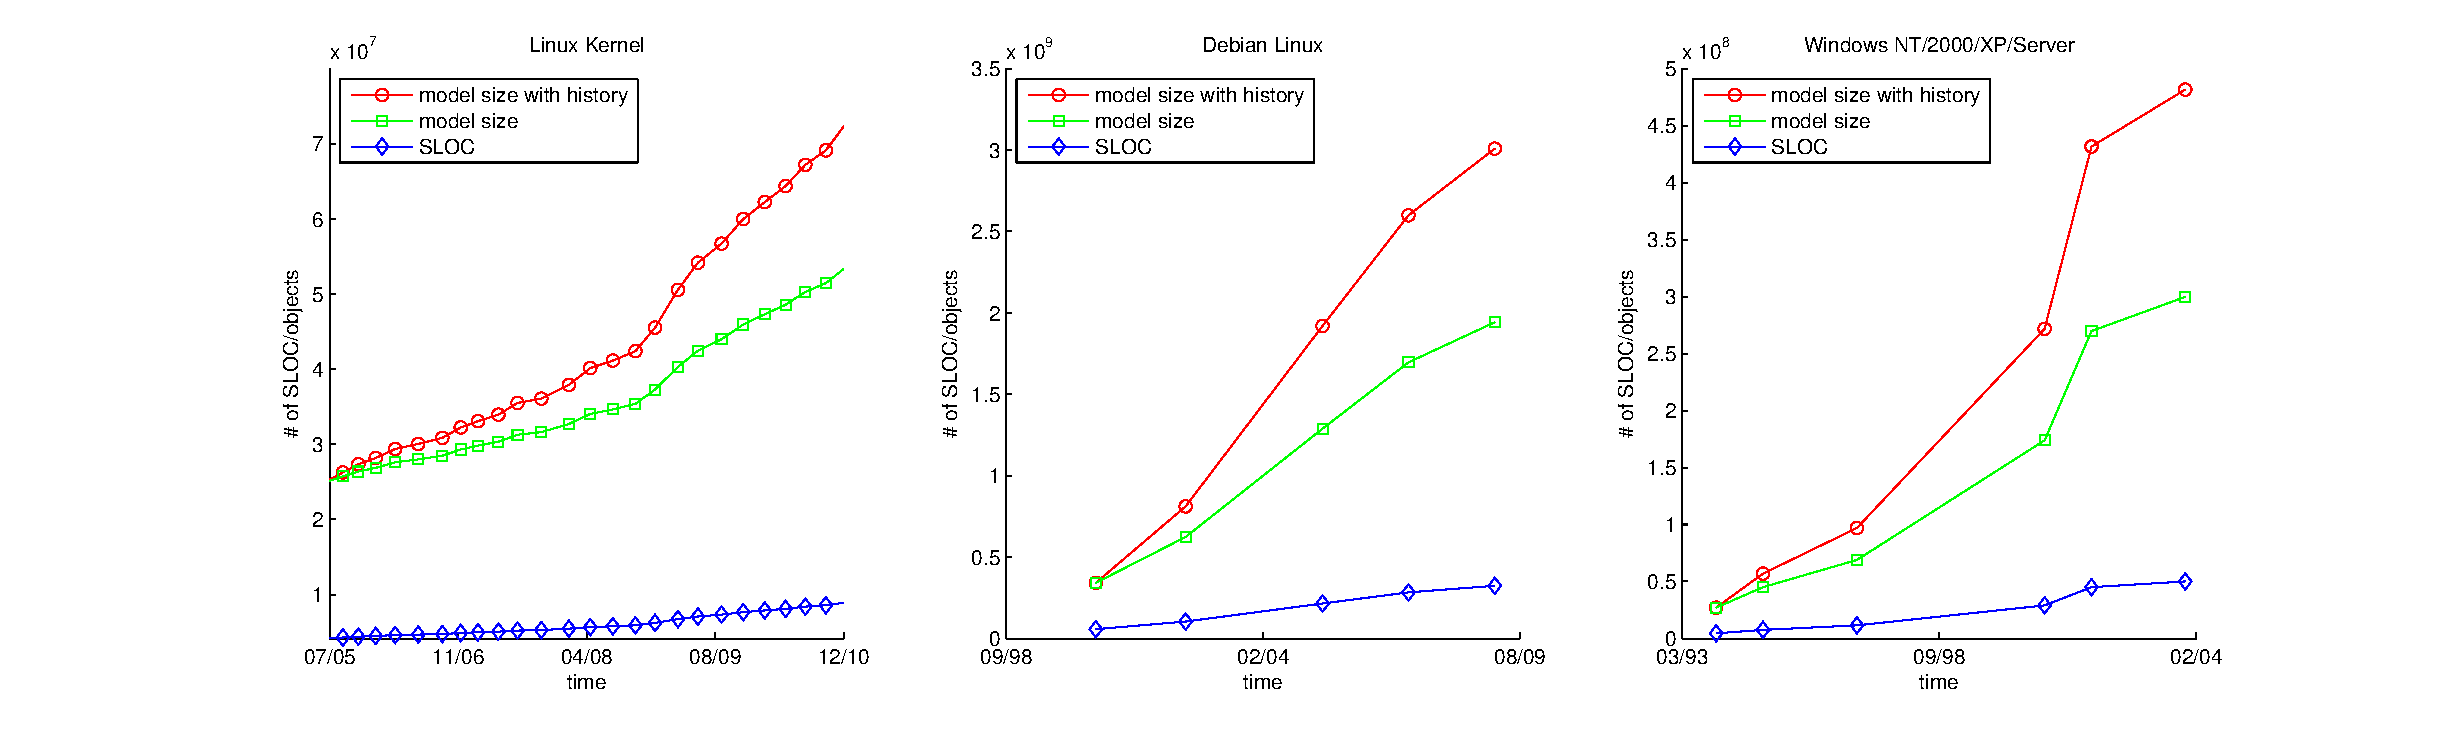
\includegraphics[width=\linewidth]{figures/software_model_sizes}
  \caption{SLOC and estimated number of objects for popular large software projects.}
  \label{fig:software_model_sizes}
\end{figure}

Fig.~\ref{fig:software_model_sizes} shows the LOC numbers and estimated object numbers in corresponding software code models. The charts present different software projects and how size developed over time. \markus{kernel, linux(debian)?, windows - numbers based on kernel git alone, SLOC numbers and transferred kernel estimates.}

\subsubsection{How big are software code models in the future?}

Some believe that the average size software (and software code models for that matter) grows faster than linear following Moore's Law. Maciej Soltysiak for example has analysed the grows of the linux kernel code base and observed exponential growth. A counter argument is that software not only bound by hardware limitations (i.e. Moore's Law) but increasingly by software complexity and therefore will not grow exponentially. Never the less, it is safe to assume that software code models will be larger in the future.


\subsection{Geospatial Models -- e.g. a 3D Model of Berlin in CityML}

\subsubsection{What are geo-spatial 3D city models?}
3D city models are a good example for structured desecrate geo spatial information. In these models geo spatial features like windows, rooms, apartments, houses, streets, boroughs, and cities are composed to form a complex graph. The CityGML standard, provides a set of xml-schemas (building upon other standards, e.g. GML) that function as a meta-model. CityGML, compared to other quasi standards (e.g. google KML) does not solely concentrate on the 3D measures, but allows to extend the covered information by more semantic attributes (e.g. materials, age, inhabitants, existing infrastructure, etc.). Geo spatial models usually come with different levels of details (LOD); CityGML distinguished 5 LODs, 0-4). 

\subsubsection{How big is an existing 3D city model?}
Like many cities, Berlin is currently establishing such a model. The current model of Berlin comprises all of Berlin, but mostly on a low-medium level of detail (LOD 1-2). To get an approximation of the model's size, we counted the XML entities. The current Berlin model, contains roughly $128*10^6$ objects. 

\subsubsection{How big will 3D city models get in the future?}
Based on data published in~\cite{CityGMLBerlinDB} a LOD 1 building comprised of 12.5 objects, a LOD 2 building of 40 objects, a LOD 3 building of 350 objects. A LOD 3-4 building of Berlin would therefore consist of $1*10^9$ objects. Berlin inhabits 3.5 million people. About 50\% of the worlds $7*10^9$ people live in cities. This gives a whole LOD3-4 approximation of $10^{12}$ objects for a \emph{world 3D city model}.

\subsection{Heterogenous Sensor Data -- e.g. HWL and Smart City}

\subsubsection{What are sensor data models?}
Sensor data usually comprises of time series of measured physical values in the environment of a sensor; but sensor data can also contain patterns of values (e.g. video images). Sensor data is collected in sensor networks, that combine distributes sensors with an communication infrastructure. Sensor data can be heterogenous: a sensor network can use different types of sensors that measure a multitude of parameters. 
\markus{cites, cites, cites}. 

We build the \emph{Humboldt Wireless Lab} are 120 node wireless sensor network. Nodes are equipped with 3 axis accelerometer, but more essentially for our research also creates data from monitoring all running software components. Components provide data as structured XML documents. Software components are themselves structures according to the software architecture.

We build a software that collects this XML data, transforms it into an EMF model, stores it in a database, and allows analysis with EMFs generated Java APIs and model transformation languages (e.g.~\cite{SMTLpaper}).

\subsubsection{How big are existing sensor data models?}
Network protocol and system software components provide 372 distinct data sets (containing data such as WLAN radio data, network statistics, CPU load levels, etc.) Each data set is represented in an XML fragment of variable size. Per second each node in the network produces XML entities that translate into an average of 1120 EMF objects. A common experiment with HWL involves 50 nodes and measures of a period of 24h. Such an experiment produces $5*10^9$ objects. 

\subsubsection{How big can sensor data models get in the future?}
Sensor networks are currently only limited by the limitations of the technical infrastructure that supports them. Will, infrastructure, and money provided, sensor networks can produce models of virtually unlimited size. 

